% small.tex
\def\tlap#1{\vbox to\z@{\vss#1}}
%\def\Tiny{\fontsize{6pt}{6pt}\selectfont}

\documentclass{beamer}
\usetheme{Berkeley}
\usecolortheme{dolphin}
\usepackage{rotating}

\title[Comparison of SAMI3 with Ionospheric Data]
{Comparison of Global Ionosonde and GPS Electron Density Measurements with the NRL SAMI3 Physics-Based Ionospheric Model during Solar Minimum}

\author{Anish Tondwalkar}
\date{\today}

\begin{document}

\maketitle
\section{Abstract}
\begin{frame}{Abstract}
  \begin{itemize}
    \item A global physics-based Ionospheric model can improve our understanding of Space Weather
      \begin{itemize}
	\item NRL SAMI3 (SAMI3 is Another Model of the Ionosphere in 3d)
      \end{itemize}
    \item Physics-based models start from “first principles”
      \begin{itemize}
	\item Climatological data and Empirical Data fits may be used
	  \begin{itemize}
	    \item e.g., Neutral Density and Winds, Solar Spectrum
	  \end{itemize}
	\item In the past, mostly used to understand physics and phenomenology
	\item Compared to ionosonde data on a global scale
      \end{itemize}
    \item Can a physics-based model simulate Space Weather? 
      \begin{itemize}
	\item Compare SAMI3 model to large Ionosonde and GPS databases of electron density measurements
	\item Start with solar quiet time (WHI)
	\item Choose locations where complex dynamics and instabilities are not affecting the data
	\item Evaluate the ``state-of-the-art''
	\item Determine if any physics is missing from SAMI3
      \end{itemize}
  \end{itemize}
\end{frame}

\section{Introduction}
\subsection{The Ionosphere}
\begin{frame}{The Ionosphere}
 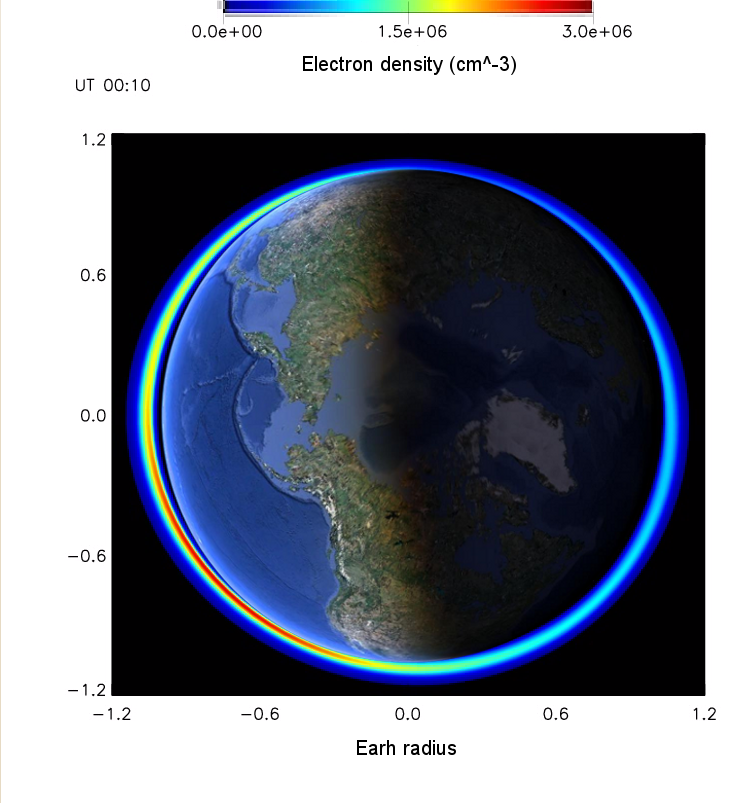
\includegraphics[height=2.0in]{planet}
 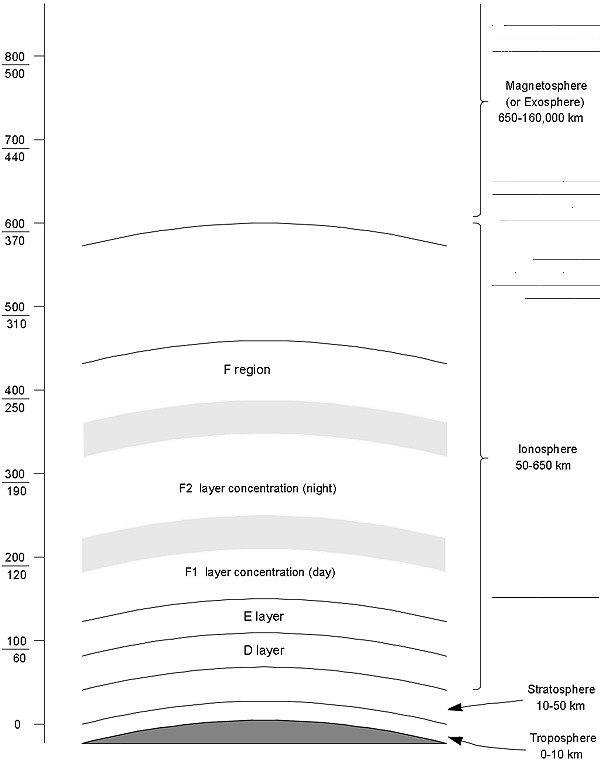
\includegraphics[height=2.0in]{layers}
\end{frame}

\begin{frame}{Why The Ionosphere?}
 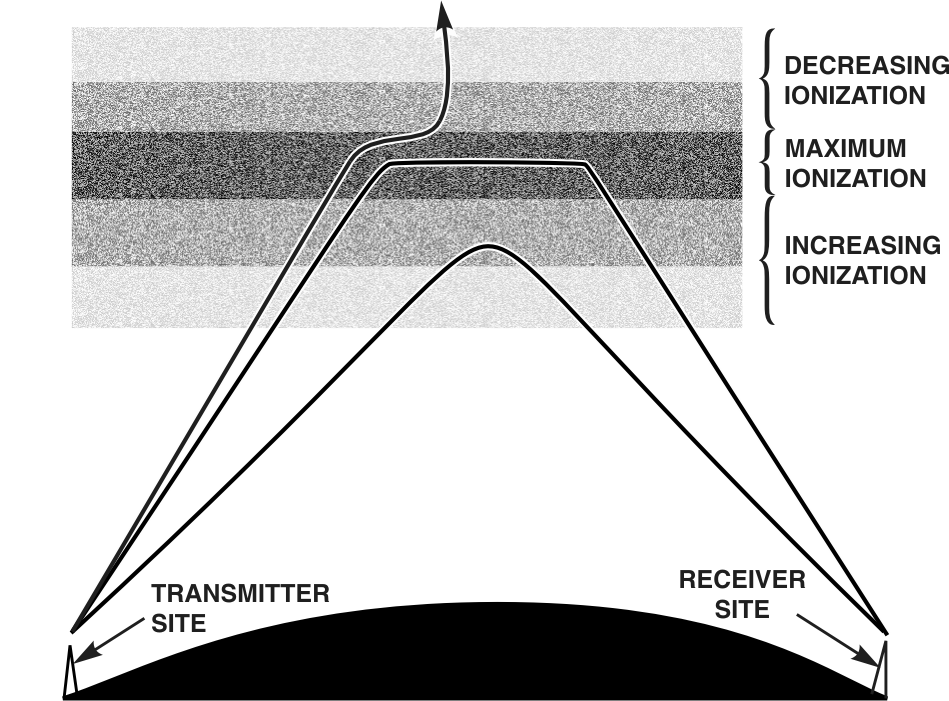
\includegraphics[height=3.0in]{bounce}
\end{frame}

%\begin{frame}{Space Weather - $A_p$, $f_{10.7}$, and $\bar f_{10.7}$}
%  \begin{columns}
%    \column{.5\textwidth}
%      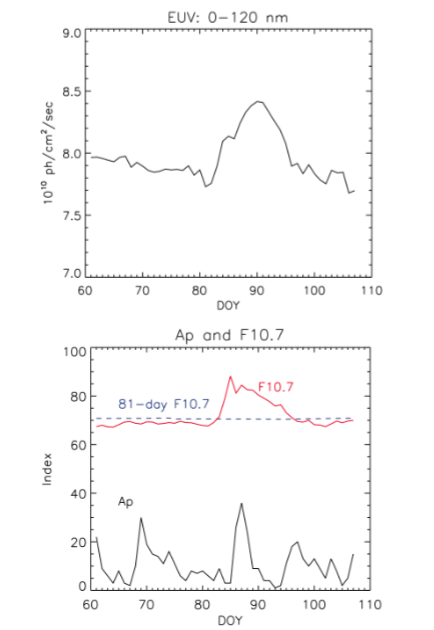
\includegraphics[height=3.0in]{space}
%    \column{.5\textwidth}
%    \begin{block}{ Note }
%     Space Weather Models are ``assimilative''. They use simplified physics to interpolate between data driven states
%    \end{block}
%  \end{columns}
%\end{frame}

\begin{frame}{It moves!}
  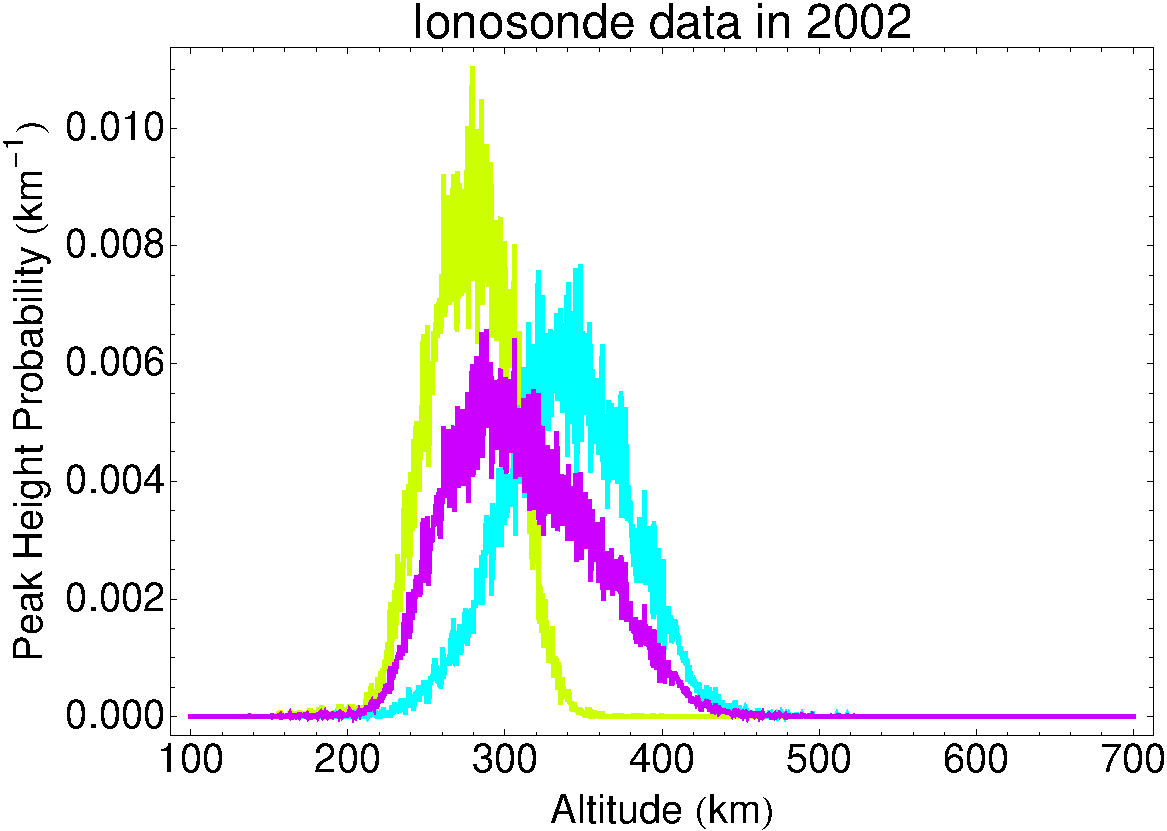
\includegraphics[height=3.0in]{plot}
\end{frame}

\begin{frame}{It moves!}
  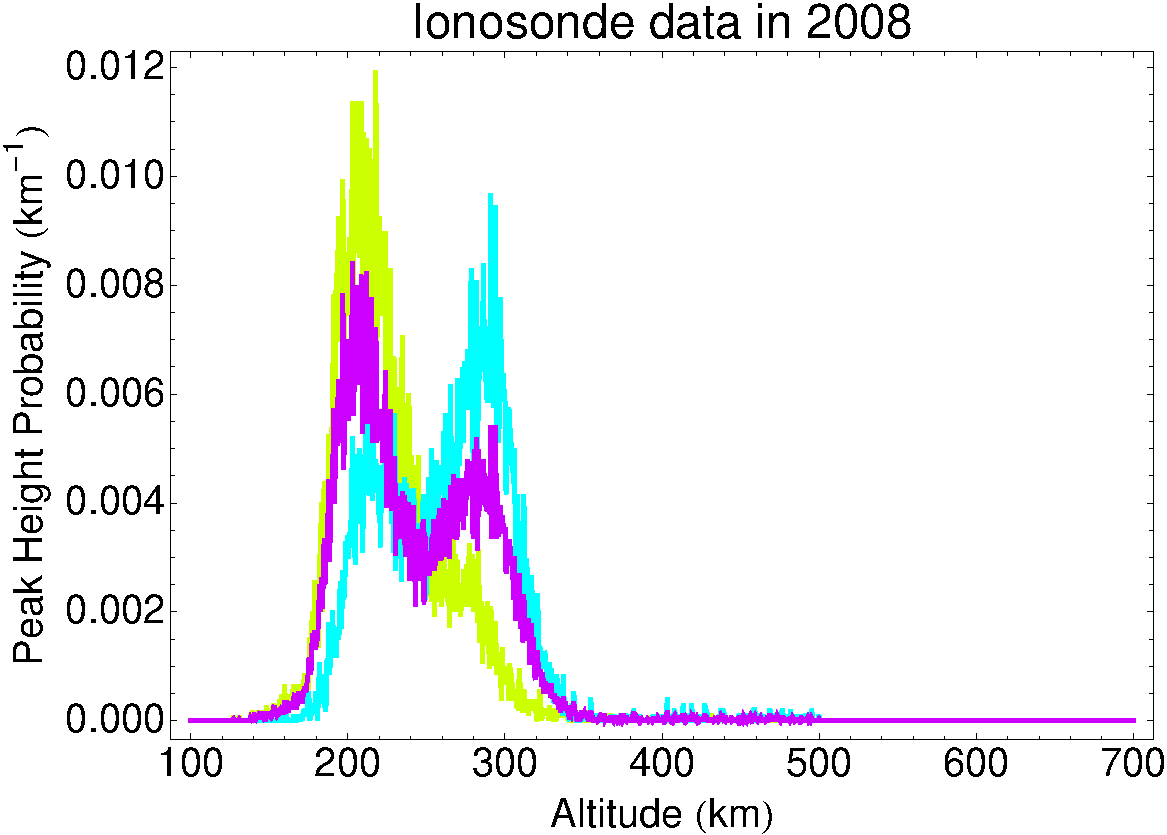
\includegraphics[height=3.0in]{2008}
\end{frame}
%\begin{frame}{What affects it?}
%  \begin{block}{}
%    \begin{tabular}[h]{p{3in}@{$\longleftrightarrow$}l}
%      $\vec E\times\vec B$ Drifts& increases $h_mF_2$ \\
%      Solar Wind and Magnetic Fields & \\
%      Neutral Winds& \\
%      Production variations (Solar EUV)& $n_mF_2$ \\
%      Recombination and Diffusion (Neutral Density) & $n_mF_2$ \\
%    \end{tabular}
%  \end{block}
%\end{frame}

\subsubsection{What affects it?}
\begin{frame}
  {Atmosphere and Ionosphere are Vertically Stratified}
  To first order the atmosphere above about 200 km can be described by the pressure/temperature scale heights.
  \begin{itemize}
    \item      Derived from Pressure and Gravity Eqilibrium $$\frac{dP}{dz} = \frac{d(nk_BT_n)}{dz} = \left< m_n \right> n_n g$$
    \item      Neutral Density $$ n_n = n_0 e^{-(z-z_0)/H_n} $$
    \item      Scale Height $$ H_n=\frac{k_B T_n}{\left<m_n\right> g} $$
  \end{itemize}
  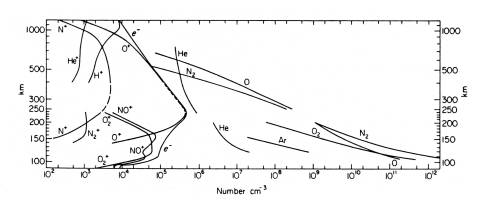
\includegraphics[height=1in,width=3in]{atmos}
\end{frame}

\begin{frame}
  {Ionization/Production}
  \begin{columns}
   \column{1.5in}
         Solar Extreme Ultraviolet (EUV)\\
          Production Rate ($P$) Depends on Solar EUV Flux ($I$) and Solar Zenith Angle ($\chi$) and Atmospheric Neutral Density ($N_n(z)$).
    $$P(\chi,z)\propto I(\chi,z) N_n(z)$$
    $P(\chi,z)$ peaks well below the $F_2$ region.
   \column{1.5in}
    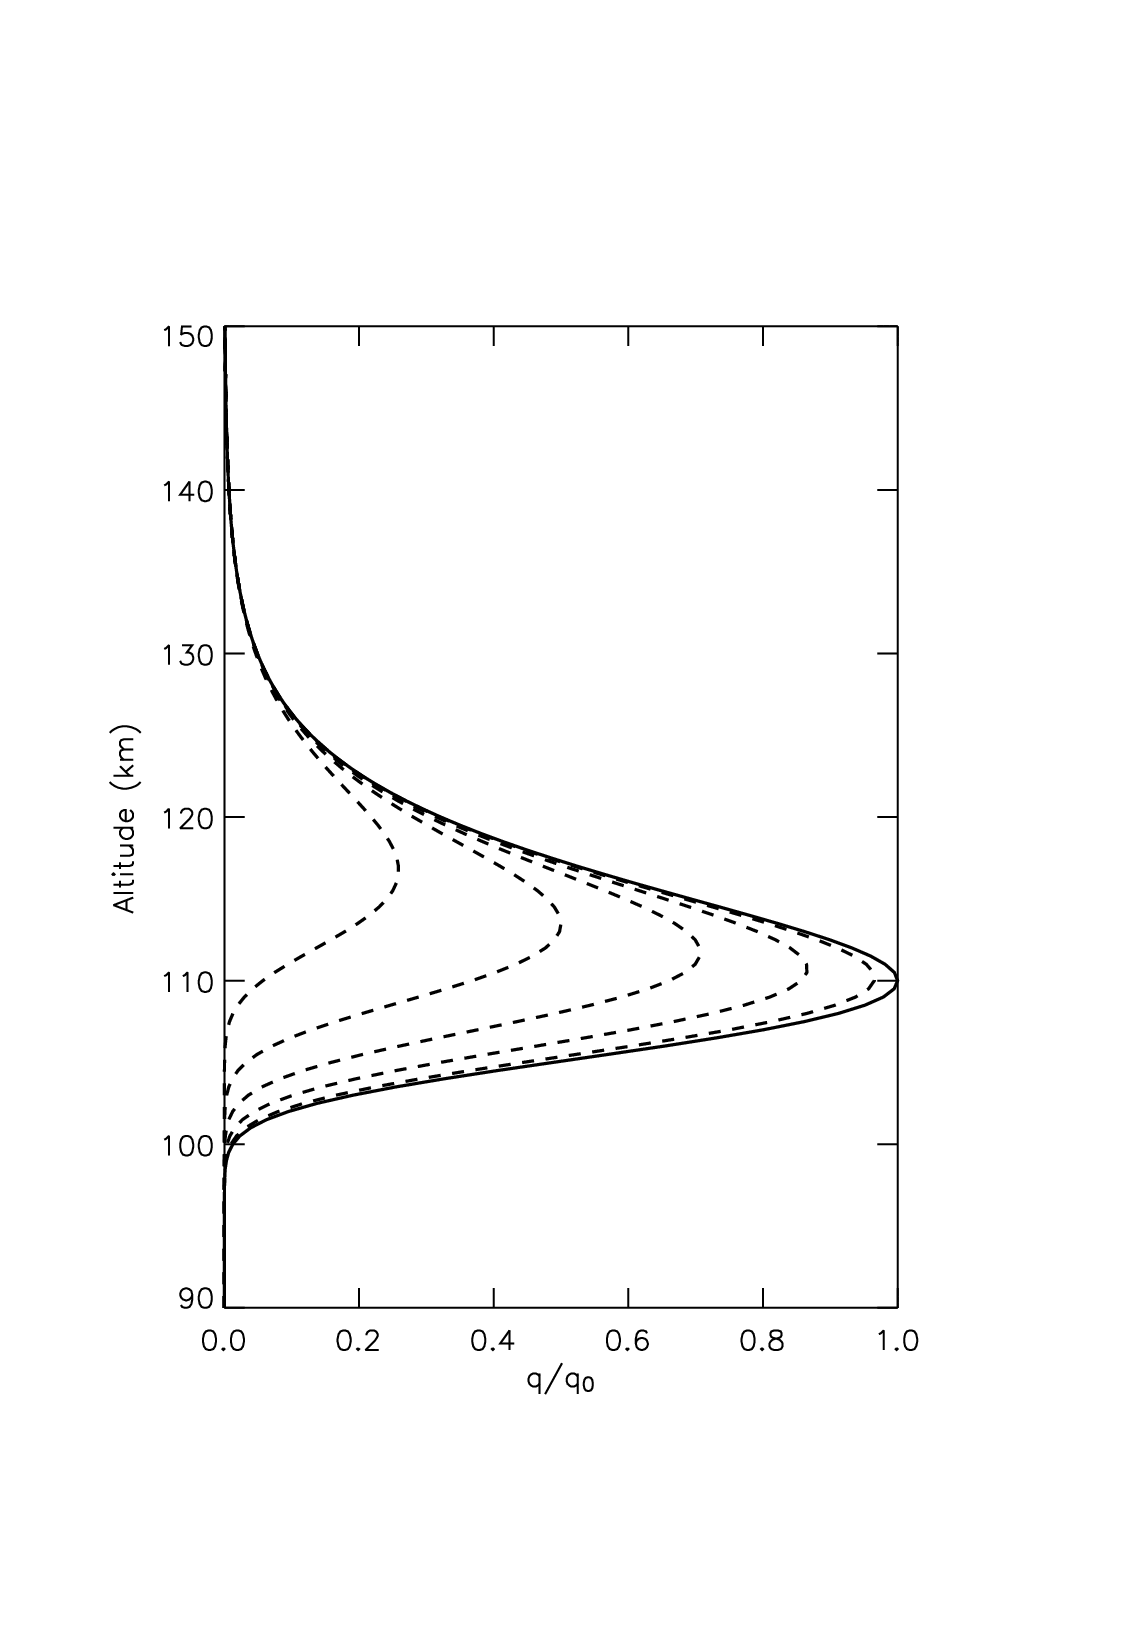
\includegraphics[height=3in]{production}
  \end{columns}
\end{frame}

\begin{frame}
  {Recombination and Diffusion}
  \begin{columns}
   \column{1.5in}\small
    Recombination and Diffusion are Ionization Loss Processes.
    The Equilibrium Electron and Ion Densities ($N_e(z)$ an $N_i(z)$) are determined by a balance of Production and Loss.
    \begin{itemize}
      \item      Both Dependent on $N_n(z)$
      \item      Peak Density $n_mF_2$ Occurs Near where Diffusion and Recombination are Equal – the Minimum Loss Condition
    \end{itemize}
   \column{1.5in}
    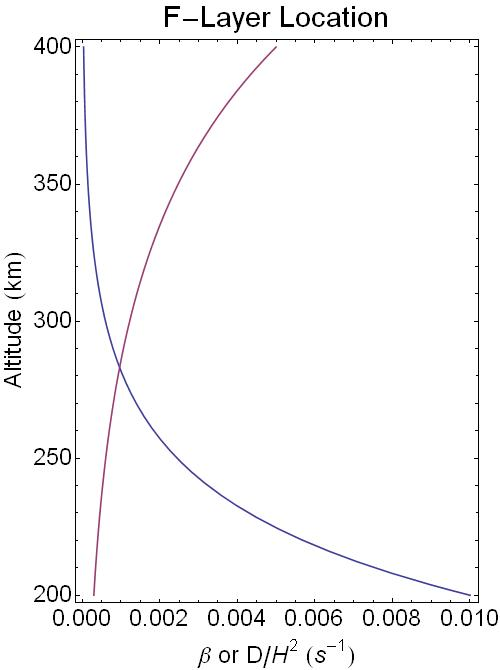
\includegraphics[height=2.5in]{loss}
  \end{columns}
\end{frame}

\begin{frame}
{Transport: ExB Drifts and Neutral Winds}
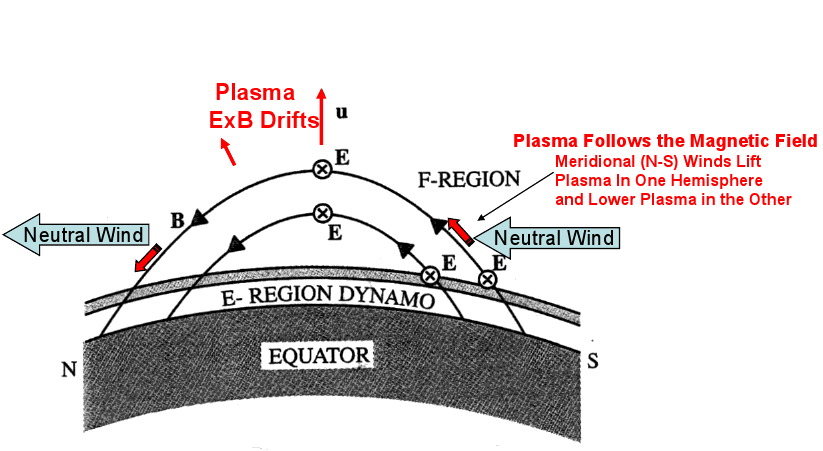
\includegraphics[width=4in]{plasma}
\end{frame}

\begin{frame}{ISES and WHI}
  \begin{block}{Integrated Sun-Earth System for the Operational Environment (ISES-OE)}
    The goal of ISES-OE is to improve our quantitative understanding of the space environment, which can disrupt or degrade operational communications and navigation systems, and ultimately to advance our ability to forecast space weather on multiple time scales.
  \end{block}
  \begin{block}{Whole Heliospheric Interval}
    Feb. 19 - April 19, 2008 contains the most recent Whole Heliospheric Interval (WHI).  This time period, during solar minimum, has only very modest solar activity and is a good test to validate the SAMI3 simulations of the base-state ionosphere.
  \end{block}
\end{frame}

\begin{frame}
  {More on WHI}
  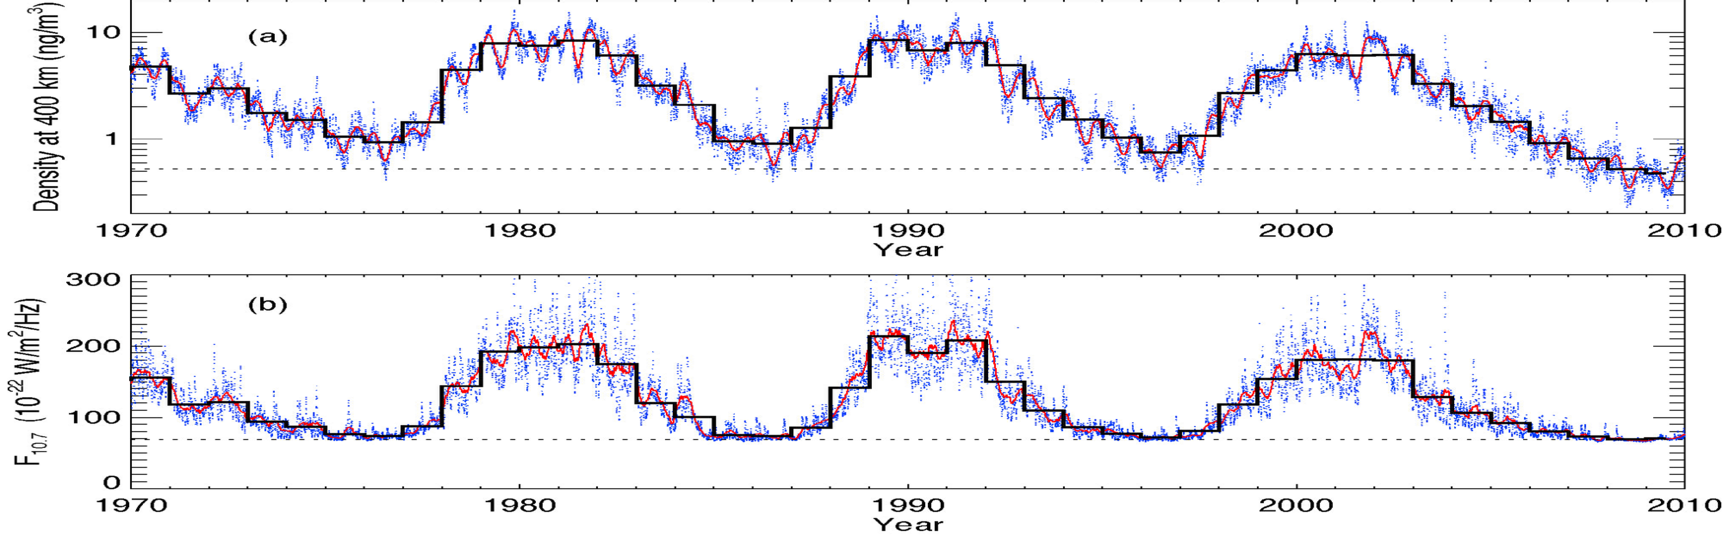
\includegraphics[width=4in,height=3in]{whi}
\end{frame}

\subsection{SAMI\{2,3\}}
\begin{frame}{SAMI}
 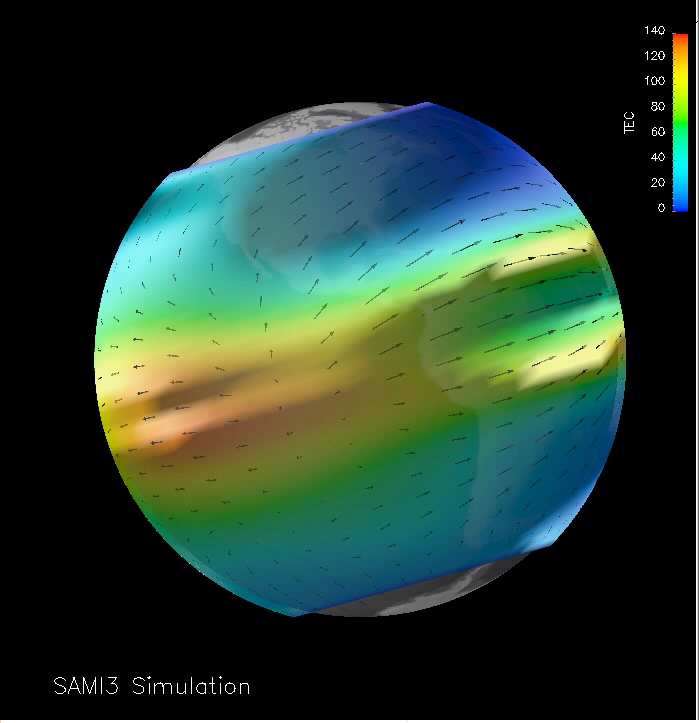
\includegraphics[height=3.0in]{SAMI}
\end{frame}

\begin{frame}{Plasma}
  \vspace{-1cm}
  \[ \omega_{pe} = \sqrt\frac{n_e e^2}{m^*\varepsilon_0} \]
  \[ \frac{\partial n_i}{\partial t} + \nabla \cdot \left( n_i\vec V_i \right) = \mathcal P_i - \mathcal L_i n_i \]
  \[ \frac{\partial \vec V_i}{\partial t} + \vec V_i \cdot \nabla \vec V_i = 
     -\frac1{\rho_i} \nabla\vec P_i 
     + \frac e{m_i}\vec E + \frac e{m_ic} \vec V_i \times \vec B 
     +\vec g \]
  \[  -\nu_{in} \left( \vec V_i -\vec V_n \right)
     -\sum_j \nu_{ij} \left( \vec V_i -\vec V_j\right) \]
  \[\frac1{n_e m_e} \nabla \vec P_e + \frac e{m_e} \vec E + \frac e{m_ec} \vec V_e \times \vec B = 0 \]
%  \[\frac{\partial T_i}{\partial{t} + \vec V_i \cdot \nabla T_i + \frac23 T_i \nabla \vec V_i 
%  +\frac23 \frac1{n_i k} \nabla \vec Q_i =Q_{in} + Q_{ii} +Q{ie} \]
\ldots and temperature equations.
\end{frame}

\begin{frame}
  {Primary SAMI3 Comparison Run}
  \begin{columns}
    \begin{column}{.5\textwidth}
      \begin{itemize}
	\item      Compensate for MSIS Departure from the atmosphere.
	\item      Exospheric Temperature is scaled by 0.960297, [O] by 0.797867, and the other neutrals by 0.969671.
      \end{itemize}
    \end{column}
      \begin{column}{.5\textwidth}
	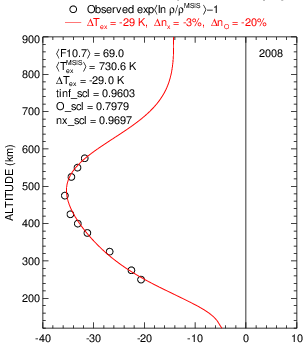
\includegraphics[height=2.2in]{cropped}\\
	Percentage Difference 
      \end{column}
  \end{columns}
\end{frame}

\subsection{Measurements}

\begin{frame}{Ionosondes and GPS}
  \begin{block}{GPS}\tiny
    By receiving GPS signals on the ground at our stations and measuring the phase and amplitude of the signal form a satellite a known distance away, we can find out the number of electrons it hit on the way here. 
  \end{block}
  \begin{block}{Ionosondes}
    \tiny Ionosondes profile density vs height.
    The transmitter sweeps all or part of the HF frequency range, transmitting short pulses. These pulses are reflected at heights of \smash{$100–400 km$},
    and the echos are received by the receiver and analyzed by the control system. The result is displayed in the form of an ionogram, a graph of reflection height (actually time between transmission and reception of pulse) versus carrier frequency.
    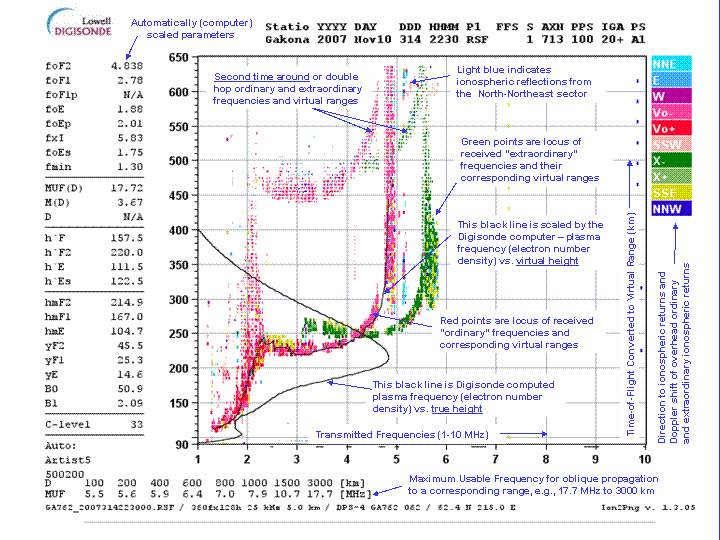
\includegraphics[width=3in]{Dsonde}
  \end{block}
\end{frame}


\section{Findings} 
\subsection{Differences by Site}
\begin{frame}{$f_oF_2 (\sim\sqrt{n_e})$}
 % \smash{\llap{\begin{sideways}
 %     Peak Freq (MHz)
 %   \end{sideways}}}
  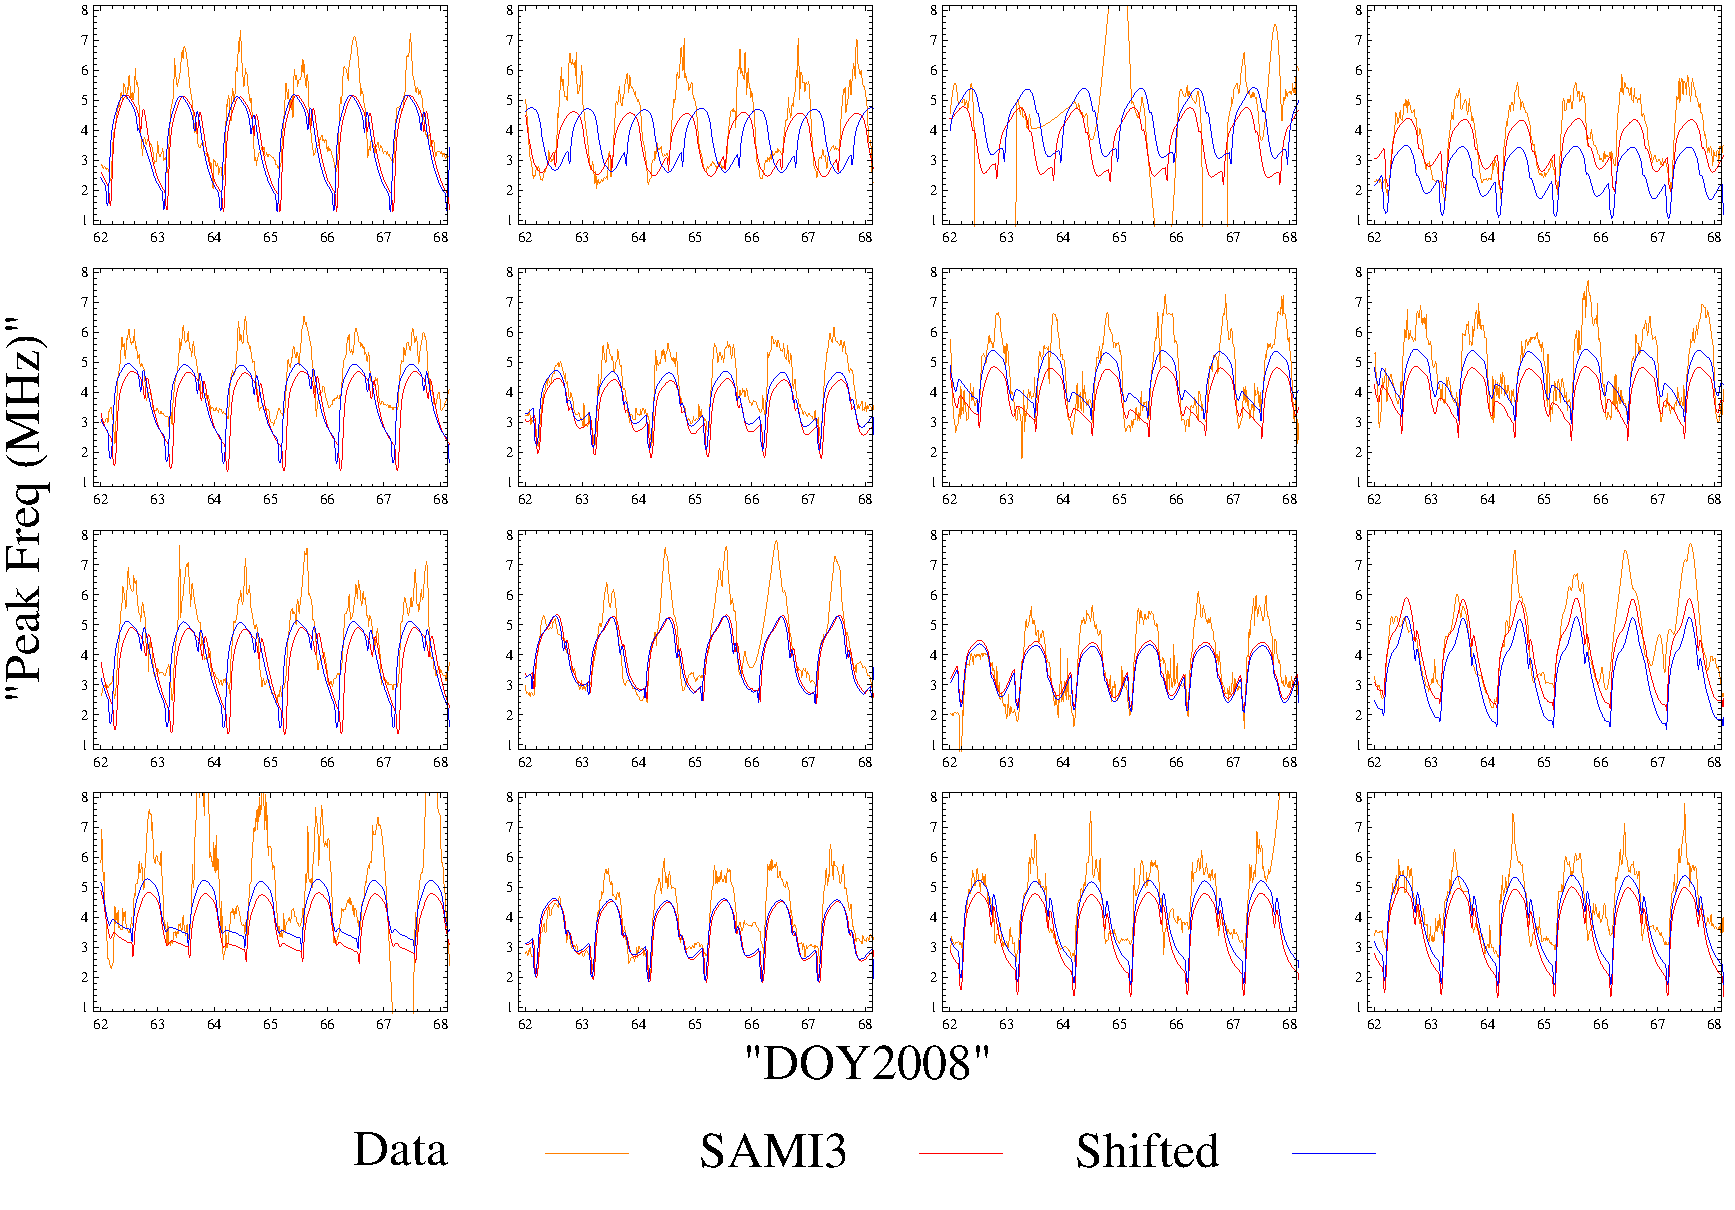
\includegraphics[width=4in]{fs}
 % \vskip -1.5in
 % \begin{center}
 %   Day
 % \end{center}
\end{frame}

\begin{frame}{$h_mF_2$}
 % \begin{sideways}
 %     Peak Height (km)
 % \end{sideways}
 % \vspace{-1.5in}
 % \hspace{1in}
  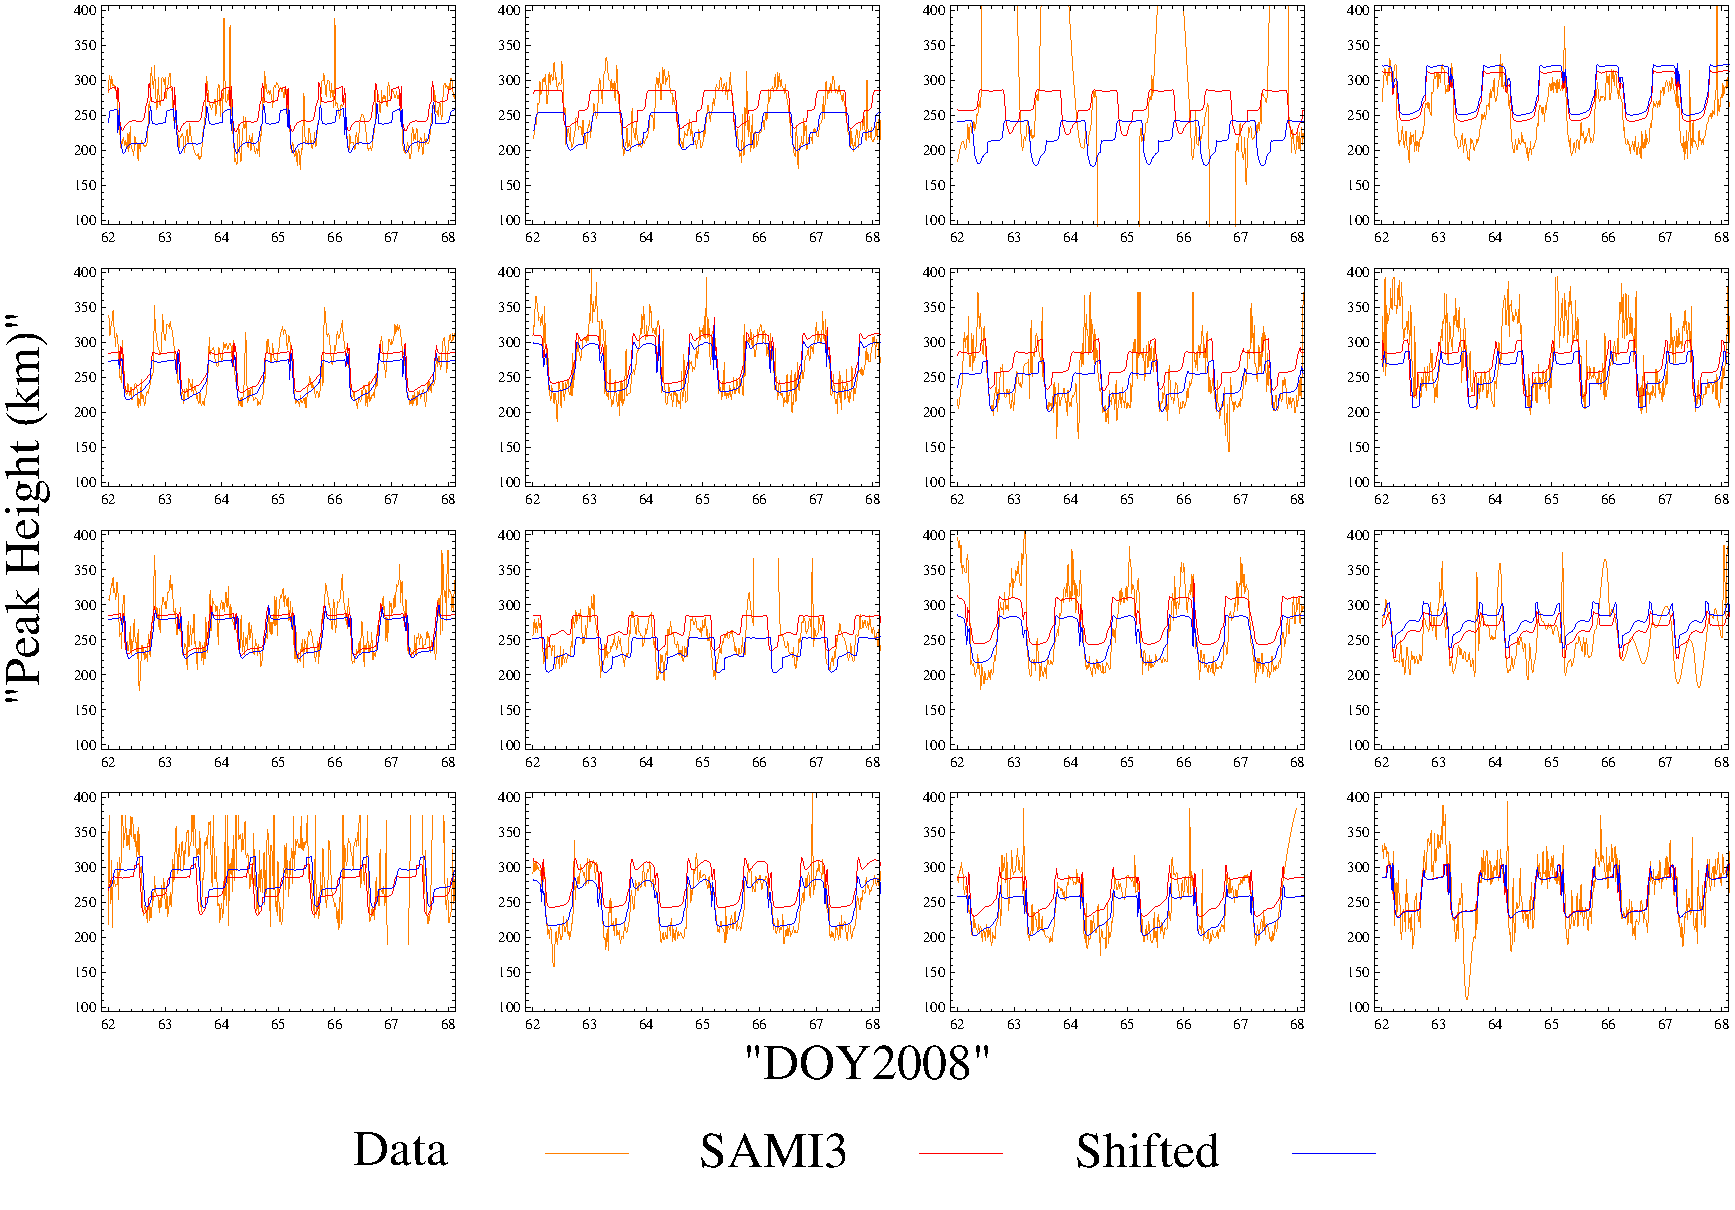
\includegraphics[width=4in]{hs}
 % \begin{center}
 %   Day
 % \end{center}
\end{frame}

\subsection{Global Differences}
\begin{frame}{Mean Global TEC}
  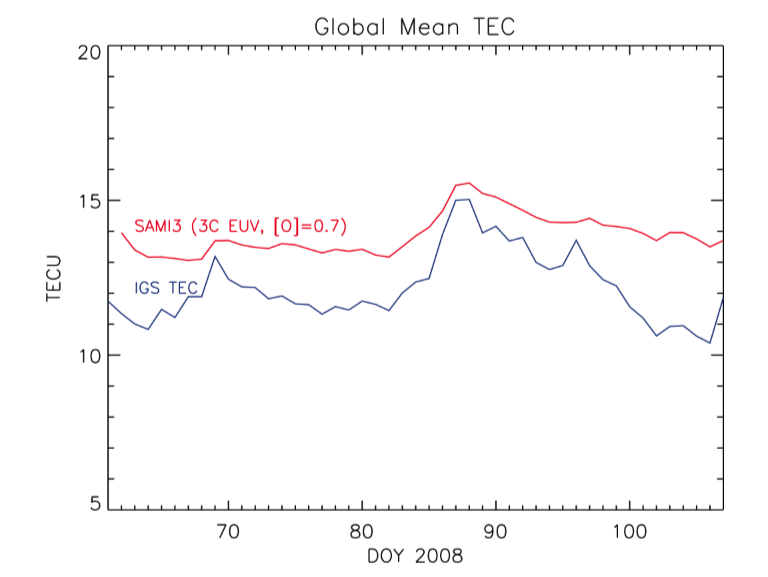
\includegraphics[height=3in]{tec}
\end{frame}

\begin{frame}{SAMI-Data Differences In Plasma Freq}
  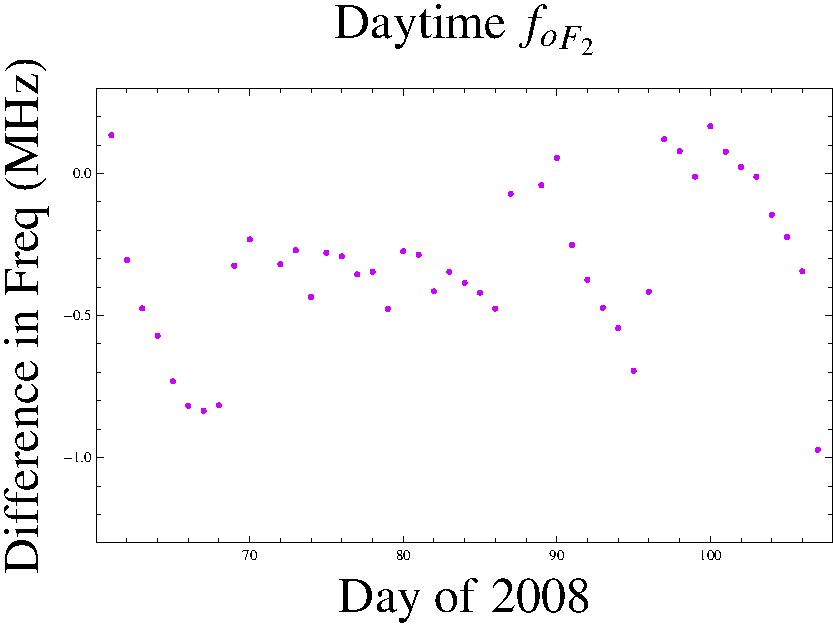
\includegraphics[height=2.5in]{dayf}
\end{frame}

\begin{frame}{SAMI-Data Differences In Plasma Freq}
  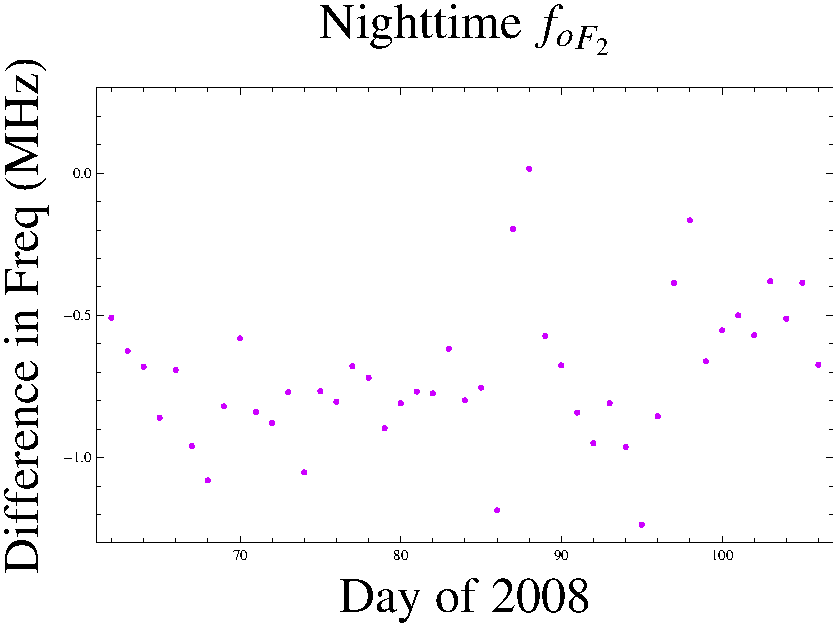
\includegraphics[height=2.5in]{nightf}
\end{frame}

\begin{frame}{SAMI-Data Differences In Peak Height}
  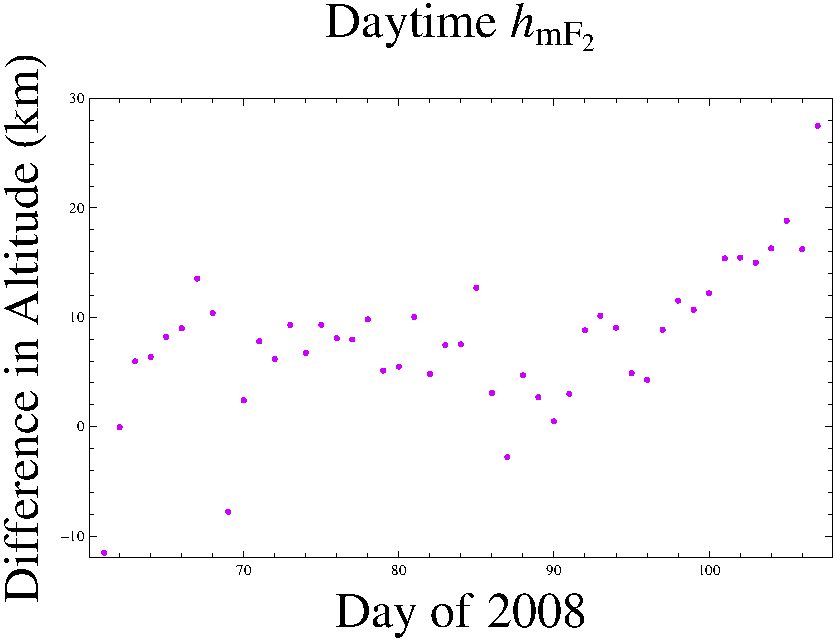
\includegraphics[height=2.5in]{dayh}
\end{frame}

\begin{frame}{SAMI-Data Differences In Peak Height}
  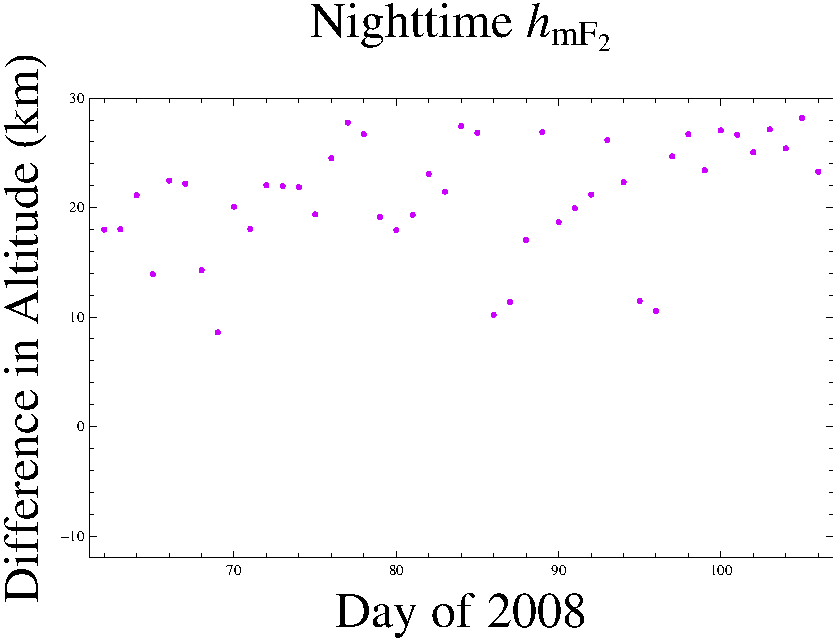
\includegraphics[height=2.5in]{nighth}
\end{frame}
 
\subsection{Modeling Experiments with SAMI2 {Effect of $T_{exo}$ and $\left[O\right]$}}
\begin{frame}{$$f_o F_2$$}
  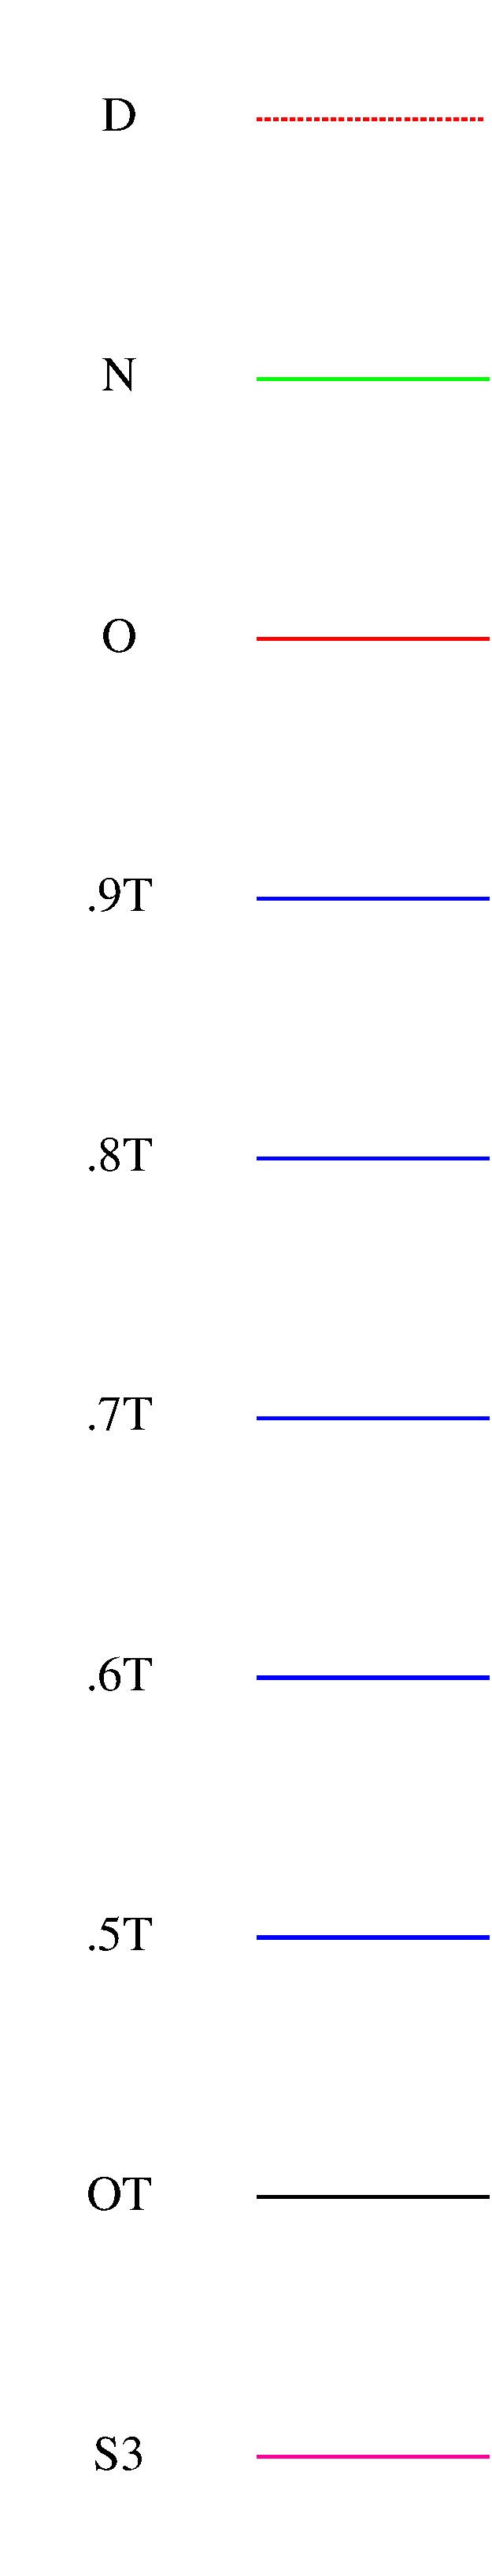
\includegraphics[height=2in]{legend}
  \includegraphics[height=2in]{fo}
\end{frame}

\begin{frame}{$$h_m F_2$$}
  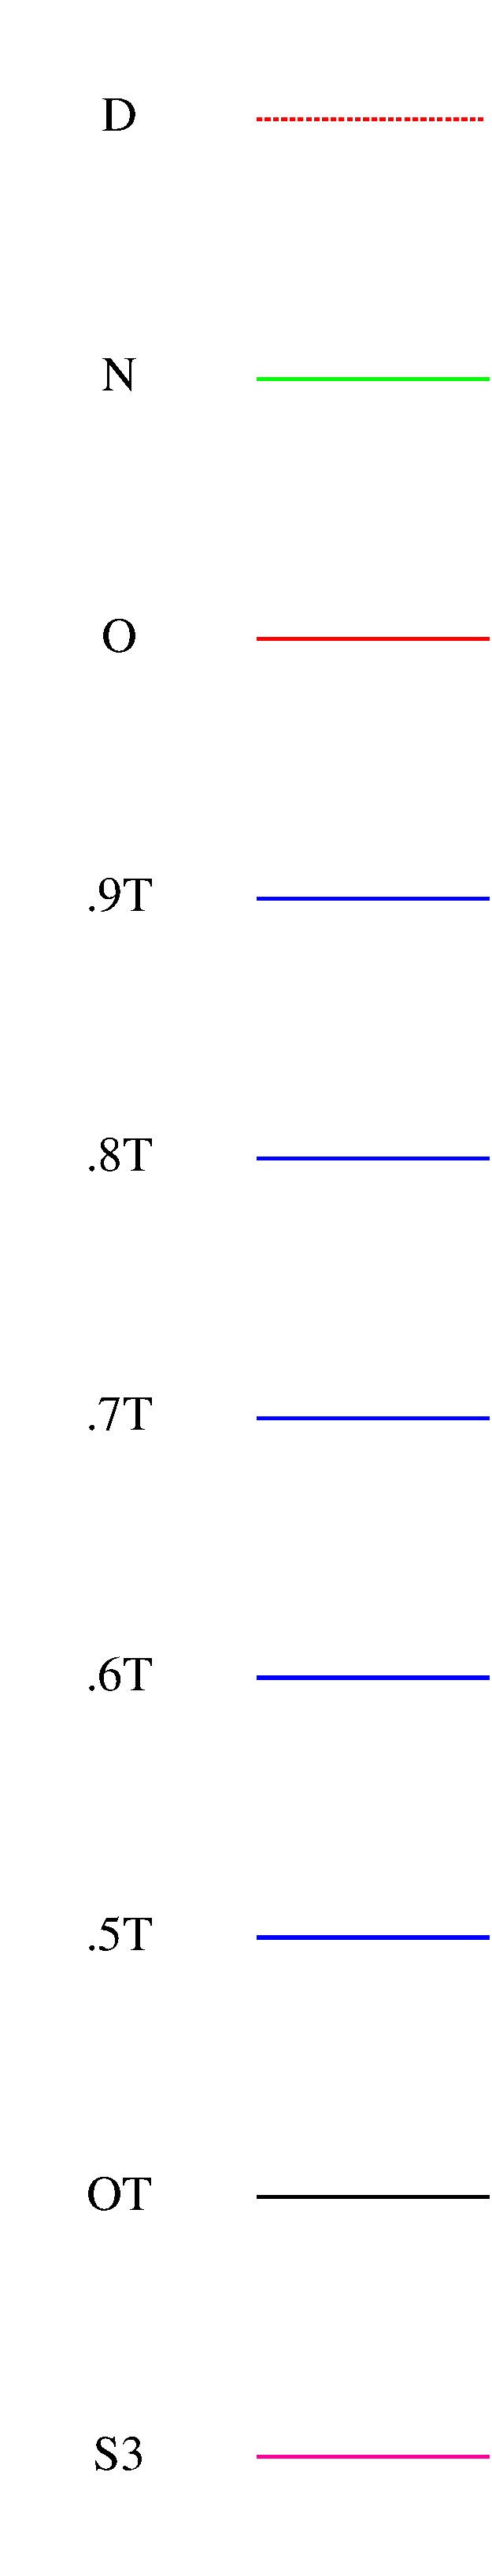
\includegraphics[height=2in]{legend}
  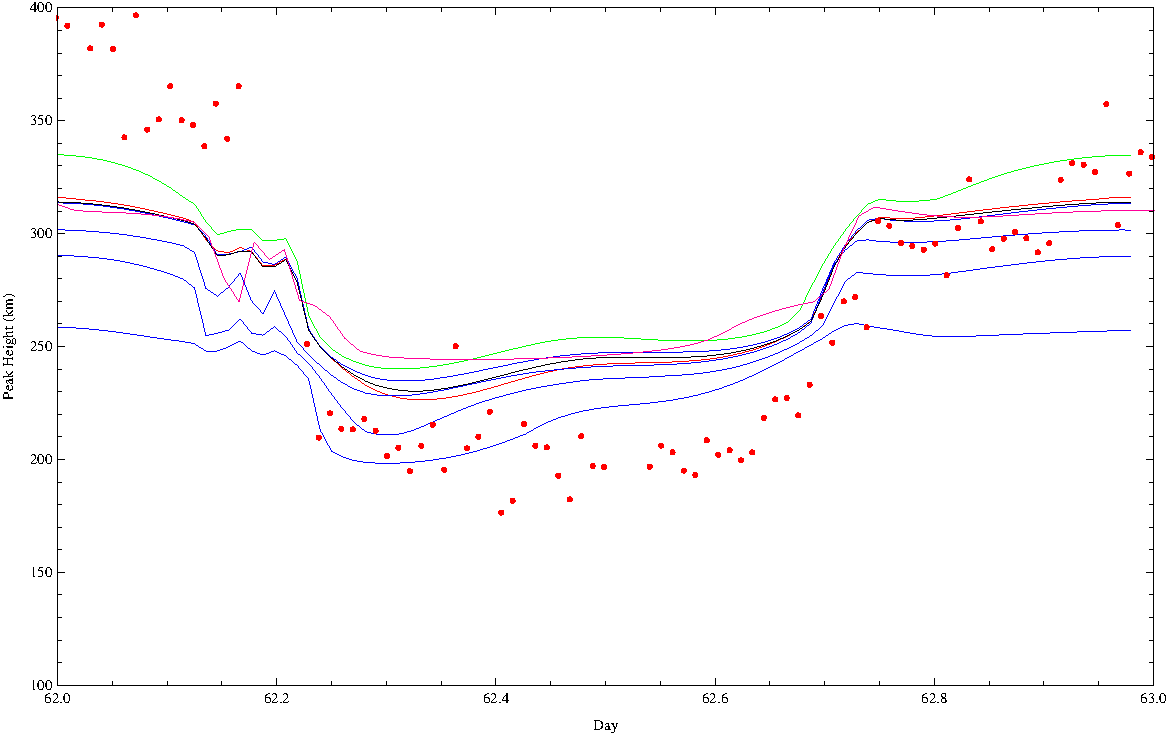
\includegraphics[height=2in]{hm}
\end{frame}


\section{Conclusion}
\begin{frame}
  {Conclusion}
%  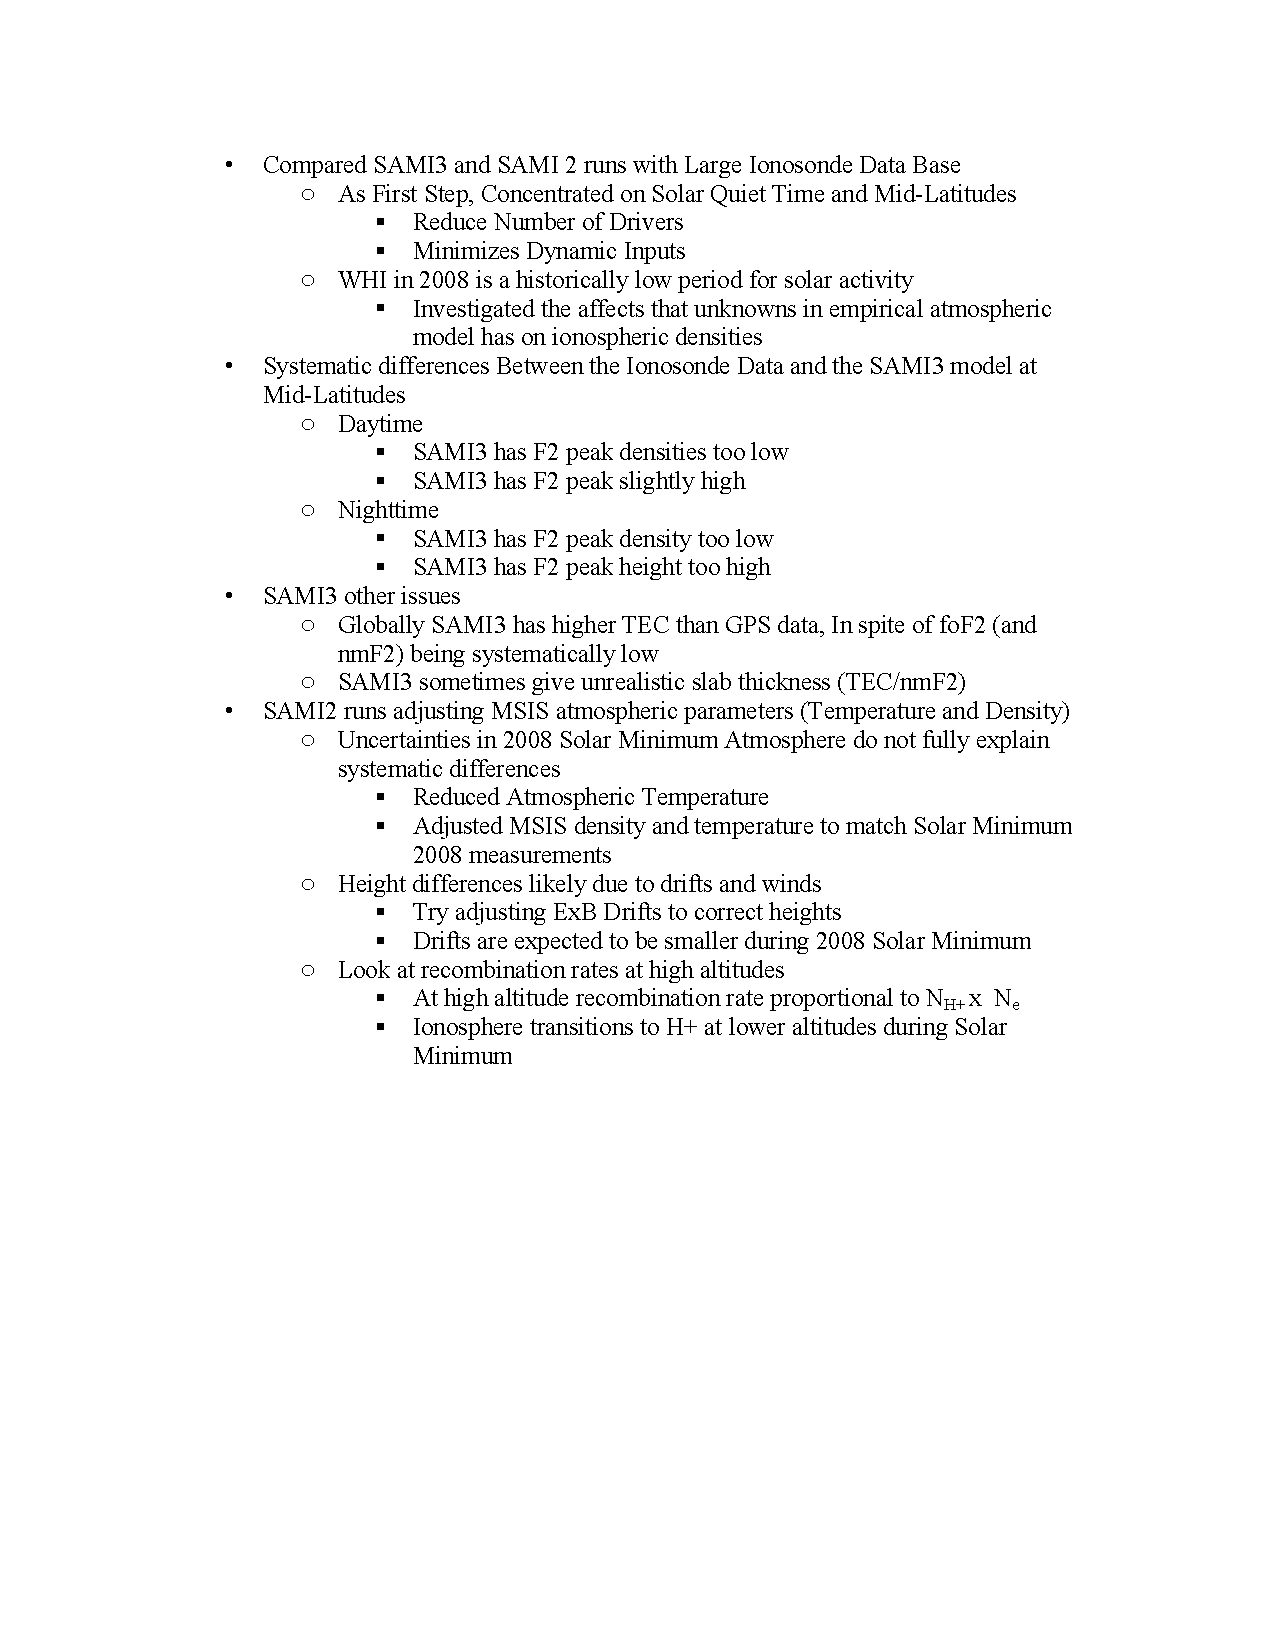
\includegraphics[width=4in,trim=0 0 363 200,clip]{sum}
\Tiny
\begin{itemize}
\Tiny
  \item    Compared SAMI3 and SAMI 2 runs with Large Ionosonde Data Base
    \begin{itemize}
\Tiny
      \item    As First Step, Concentrated on Solar Quiet Time and Mid-Latitudes
	\begin{itemize}
\Tiny
	  \item    Reduce Number of Drivers
	  \item    Minimizes Dynamic Inputs
	\end{itemize}
      \item    WHI in 2008 is a historically low period for solar activity
	\begin{itemize}
\Tiny
	  \item    Investigated the affects that unknowns in empirical atmospheric model has on ionospheric densities
	\end{itemize}
    \end{itemize}
  \item    Systematic differences Between the Ionosonde Data and the SAMI3 model at Mid-Latitudes
    \begin{itemize}
\Tiny
      \item    Daytime
	\begin{itemize}
\Tiny
	  \item    SAMI3 has F2 peak densities too low 
	  \item    SAMI3 has F2 peak slightly high
	\end{itemize}
      \item    Nighttime
	\begin{itemize}
\Tiny
	  \item    SAMI3 has F2 peak density too low
	  \item    SAMI3 has F2 peak height too high
	\end{itemize}
    \end{itemize}
  \item    SAMI3 other issues
    \begin{itemize}
\Tiny
      \item    Globally SAMI3 has higher TEC than GPS data, In spite of foF2 (and nmF2) being systematically low
      \item    SAMI3 sometimes give unrealistic slab thickness (TEC/nmF2)
    \end{itemize}
  \item    SAMI2 runs adjusting MSIS atmospheric parameters (Temperature and Density)
    \begin{itemize}
\Tiny
      \item    Uncertainties in 2008 Solar Minimum Atmosphere do not fully explain systematic differences
	\begin{itemize}
\Tiny
	  \item    Reduced Atmospheric Temperature 
	  \item    Adjusted MSIS density and temperature to match Solar Minimum 2008 measurements
	\end{itemize}
      \item    Height differences likely due to drifts and winds
	\begin{itemize}
\Tiny
	  \item    Try adjusting ExB Drifts to correct heights
	  \item    Drifts are expected to be smaller during 2008 Solar Minimum
	\end{itemize}
      \item    Look at recombination rates at high altitudes
	\begin{itemize}
\Tiny
	  \item    At high altitude recombination rate proportional to NH+ x  Ne
	  \item    Ionosphere transitions to H+ at lower altitudes during Solar Minimum
	\end{itemize}
    \end{itemize}
\end{itemize}
\end{frame}

\begin{frame}{Acknowledgements}
 I'd like to thank Dr. Paul Bernhardt, Dr. Jonathan Krall and my mentor Dr. Carl Siefring.
\end{frame}

\end{document}
